\section*{Introduction}
In this report an autopilot for a cargo ship is developed, and a discrete Kalman filter is applied to the system. To obtain desirable results, stochastic modeling, basic identification and control theory are all used. The entire project is run through Mathworks powerful software MatLab as a simulation of a real system. Graphs, Simulink models and Matlab code are all a part of this report, explaining and displaying our results.


\section{Identification of Boat Parameters}
In this section a transfer function from the rudder input $\delta$ to the average heading $\psi$ is derived for the ship. The simulation model provides estimated parameters for the transfer function, before a comparison between the response of the transfer function and the simulation model is made to evaluate the approximation.


%%%%%%%%%%%%%%%%%%%%%%%%%%%%%%%%%%%%%%%%%%%%%%%%%%%%%%%%%%%%%%%%%%%%%%%%
% 1.1 Transfer Function
%%%%%%%%%%%%%%%%%%%%%%%%%%%%%%%%%%%%%%%%%%%%%%%%%%%%%%%%%%%%%%%%%%%%%%%%
\subsection{Transfer function}
In order to derive a transfer function from $\delta$ to $\psi$, the we will have to assume no current disturbances, using the equations for $\dot{\psi}$ and $\dot{r}$ given by:

\begin{equation}\label{Average Heading}
    \dot{\psi} = r
\end{equation}

\begin{equation}\label{Derived r}
    \dot r =  - \frac{1}{T}r + \frac{K}{T}\delta  
\end{equation}

The model for the average heading is obtained by inserting (\ref{Derived r}) into the derivative of (\ref{Average Heading})

\begin{equation}\label{dDerived psi}
    \ddot \psi  =  - \frac{1}{T}r + \frac{K}{T}\delta 
\end{equation}

The transfer function from $\delta$ to $\psi$ is obtained by applying Laplace-transformation to (\ref{dDerived psi}), assuming zero initial conditions.

\begin{equation}\label{Transfer function}
    H(s) = \frac{{\psi (s)}}{{\delta (s)}} = \frac{K}{{s(Ts + 1)}}
\end{equation}

The transfer function (\ref{Transfer function}) describes how the rudder ($\delta$) affects the average heading ($\psi$).


%%%%%%%%%%%%%%%%%%%%%%%%%%%%%%%%%%%%%%%%%%%%%%%%%%%%%%%%%%%%%%%%%%%%%%%%
% 1.2 Identifying Boat Parameteres without Disturbances
%%%%%%%%%%%%%%%%%%%%%%%%%%%%%%%%%%%%%%%%%%%%%%%%%%%%%%%%%%%%%%%%%%%%%%%%
\subsection{Identifying Boat Parameteres without Disturbances}

To obtain the values of K and T from (\ref{Transfer function}), we applied two sine inputs of different frequency to the simulation, observing the amplitude of the output. By using the fact that

\begin{equation}\label{A0Ai}
    {A}\left| {H(j{\omega _i})} \right| = {A_0}
\end{equation}

where $A$ is the amplitude and $\omegA$ is the frequency of the input signal, while $A_0$ is the amplitude of the output signal. This method provides a set of two equations with the same number of unknown variables, which we solved for T and K.

Expanding equation (\ref{A0Ai}) gives:
    
\begin{equation}\label{Hjw}
        \left| {H(j{\omega _i})} \right|{A} = \frac{{\left| K \right|}}{{\left| { - T{\omega ^2} + j\omega } \right|}}{A} = {A_0}
\end{equation}

\begin{equation}\label{K}
    K = \omega \sqrt {{T^2}{\omega ^2} + 1\frac{{{A_0}}}{{{A}}}}
\end{equation}

\begin{equation}\label{T}
    T = \sqrt {\frac{{{K^2}}}{{{\omega ^4}}}\frac{{{A}^2}}{{{A_0}^2}} - \frac{1}{{{\omega ^2}}}}
\end{equation}

Now we have isolated K and T. Next we are denoting $\omega$ and $A_0$ in equation (\ref{K}) and (\ref{T}) respectively to $\omega_1$ along with $A_{01}$ and $\omega_2$ along with $A_{02}$. This provides the following expression for K:

\begin{equation}
    K = {\omega _1}\sqrt {\left( {\frac{{{K^2}}}{{{\omega _2}^4}}\frac{{{A}^2}}{{{A_{{0_2}}}^2}} - \frac{1}{{{\omega _2}^2}}} \right){\omega _1}^2}  + 1\frac{{{A_{{0_1}}}}}{{{A}}}
\end{equation}

\begin{equation}\label{K_calc}
    K = \sqrt {\frac{{{A_{{0_1}}}^2{\omega _1}^2 - \frac{{{\omega _1}^4{A_{{0_1}}}^2}}{{{\omega _2}^2}}}}{{1 - \frac{{{\omega _1}^2{A_{{0_1}}}^2{A}^2}}{{{\omega _2}^4{A_{{0_2}}}^2}}}}}  \cdot \frac{1}{{{A}}}
\end{equation}

The values for $A_{01}$ and $A_{02}$ are obtained by running the simulation without disturbances including the following constants:

\begin{align*}
\omega_1 &= 0.005\\
\omega_2 &= 0.05\\
A &= 1
\end{align*}

\begin{figure}[!htb]
    \caption{Average heading without disturbances A=1}
    \centering
    \centerline{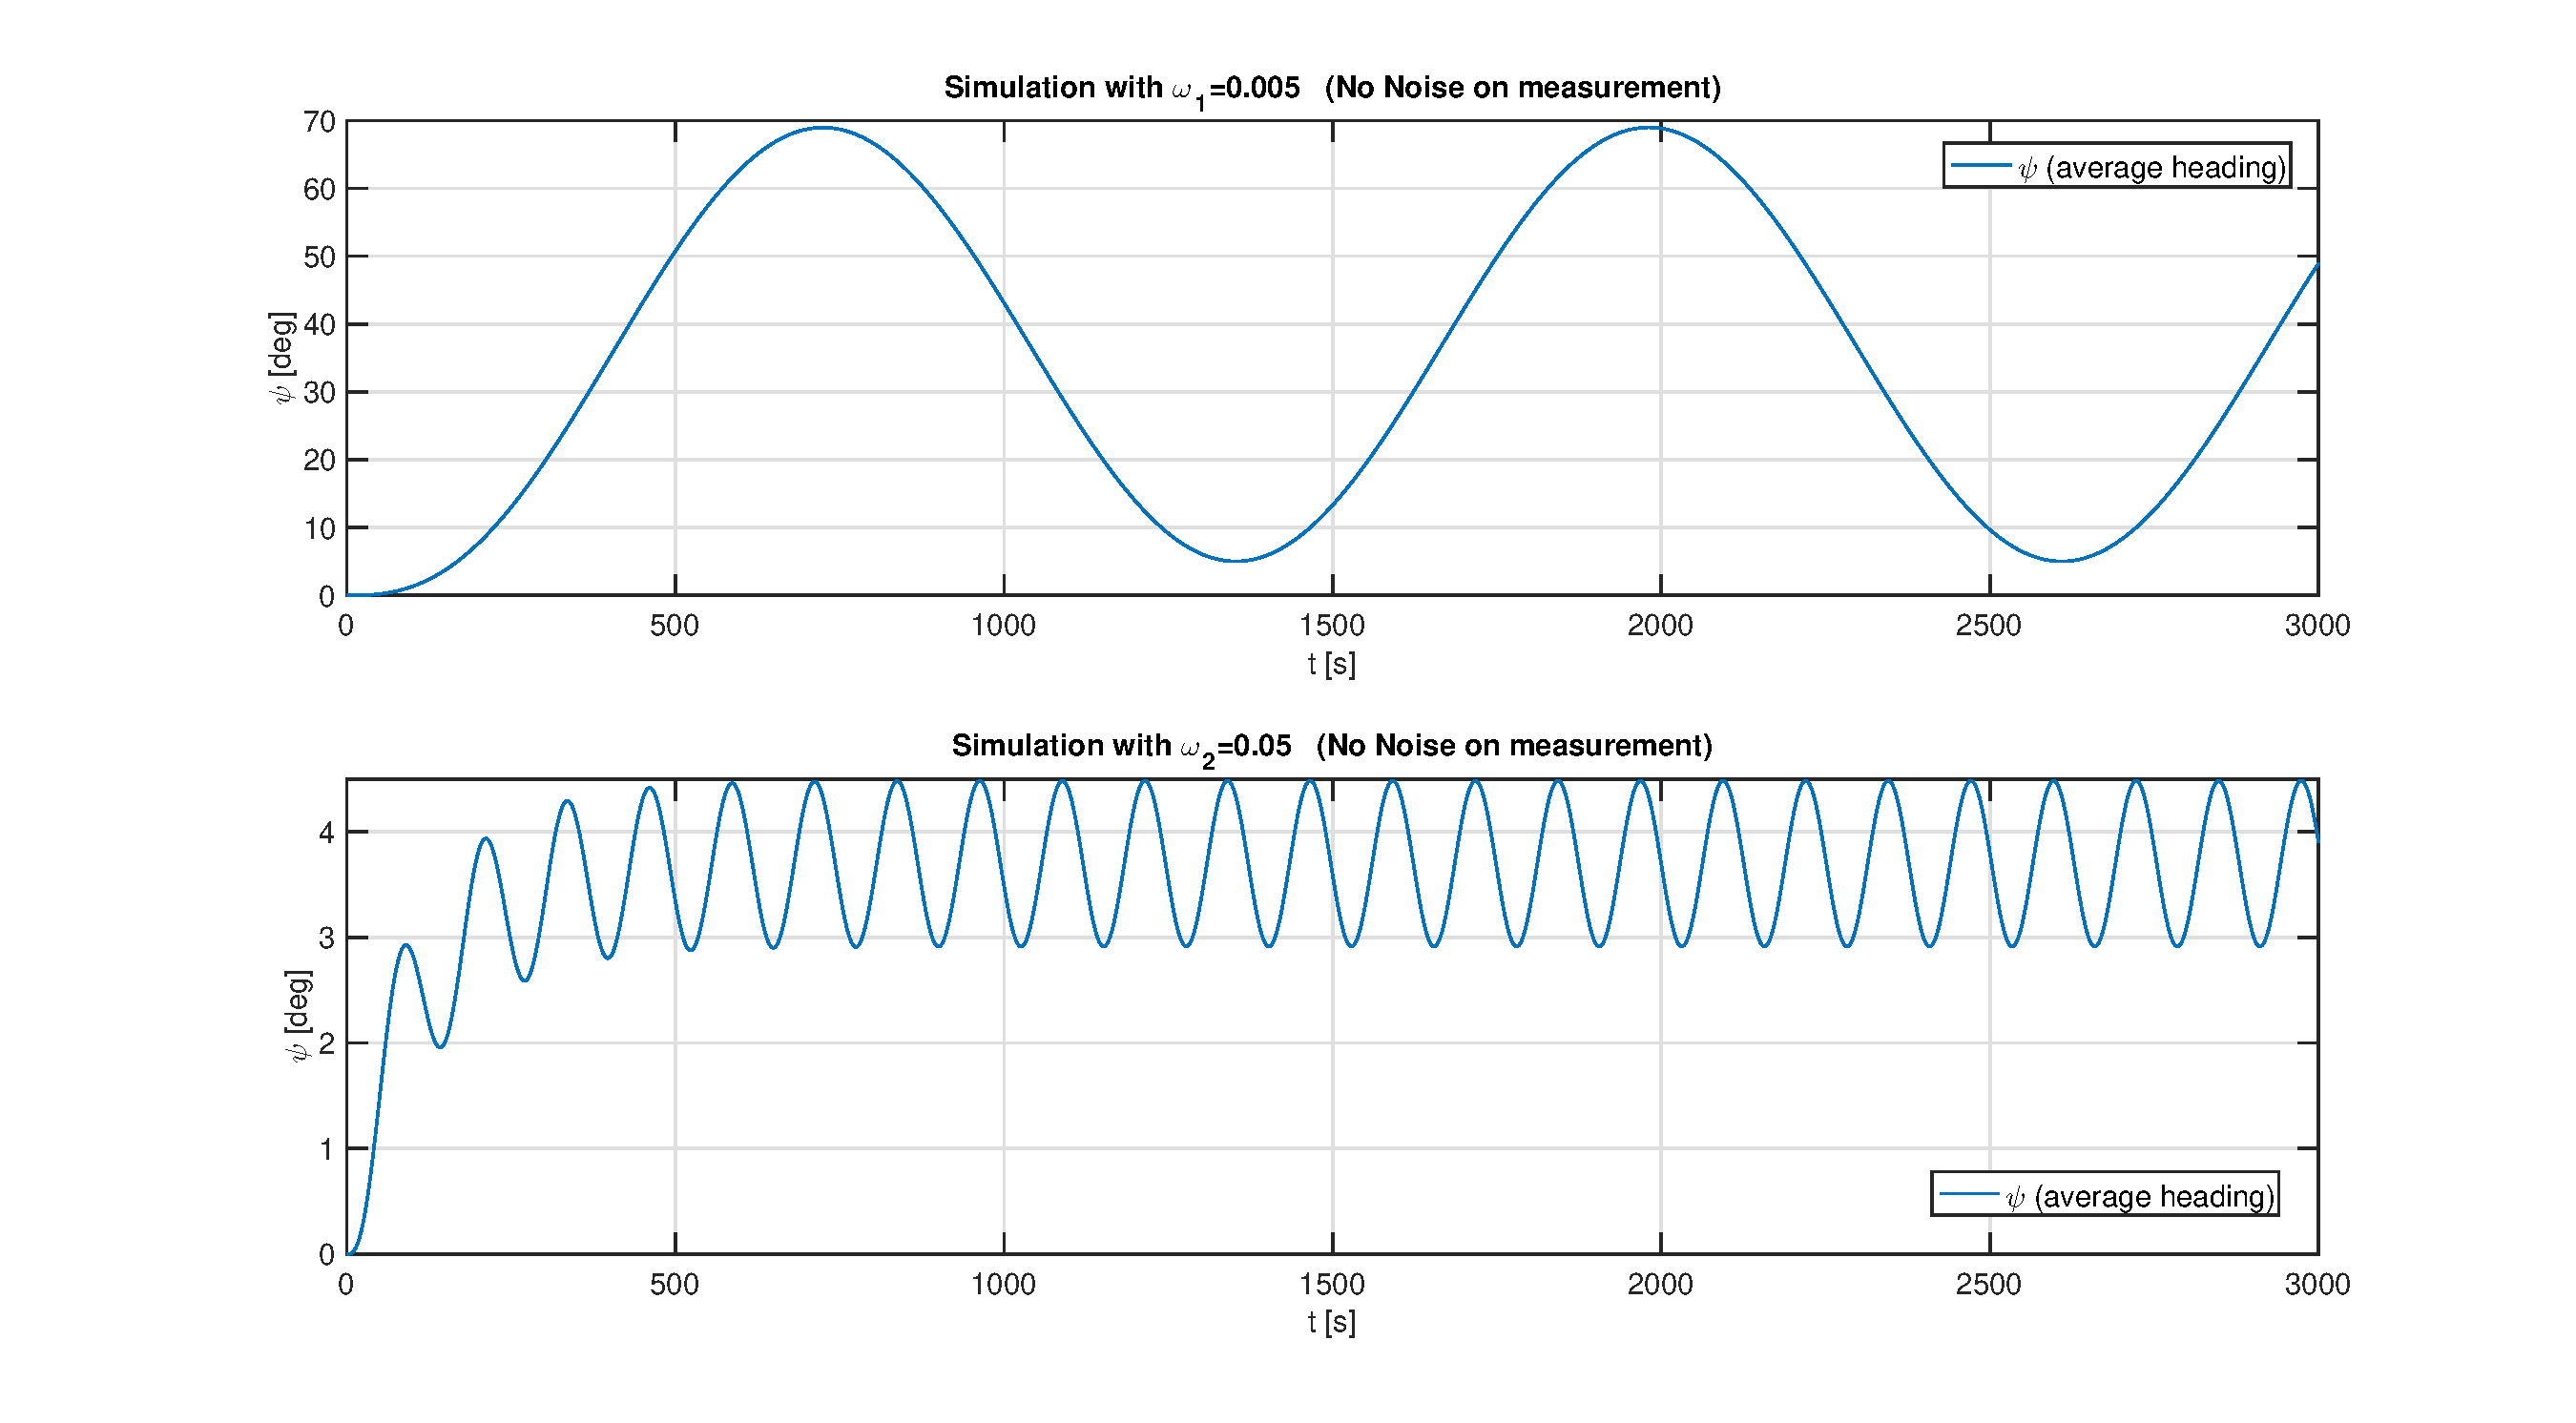
\includegraphics[scale=0.4]{plots/1b}}
\end{figure}





From figure 1 we extract the amplitude of the outputs, respectively $A_{01}$ and $A_{02}$, which are found by reading and inserting the maximum and minimum values as shown below:

\begin{align*}
{A_{{0_1}}}  &= \frac{{68.98 - 5.02}}{2} = 31.98\\
{A_{{0_2}}} &= \frac{{4.48 - 2.92}}{2} = 0.78
\end{align*}

Inserting these values into equation (\ref{T}) and equation (\ref{K_calc}) gives:

\begin{align*}
K  &= 0.1742\\
T &= 86.5268
\end{align*}







%%%%%%%%%%%%%%%%%%%%%%%%%%%%%%%%%%%%%%%%%%%%%%%%%%%%%%%%%%%%%%%%%%%%%%%%
% 1.3 Boat Parameters with Wave and Measurement Noise
%%%%%%%%%%%%%%%%%%%%%%%%%%%%%%%%%%%%%%%%%%%%%%%%%%%%%%%%%%%%%%%%%%%%%%%%
\subsection{Boat Parameters with Wave and Measurement Noise}

In this section, the previous section will be repeated, but with disturbance. The disturbance consists of waves and measurement noise. Figure 2 displays the output when $\omega = \omega_{1}$ and when $\omega = \omega_{2}$.

\begin{figure}[!htb]
    \caption{Average heading with waves and measurment noise, A=1}
    \centering
    \centerline{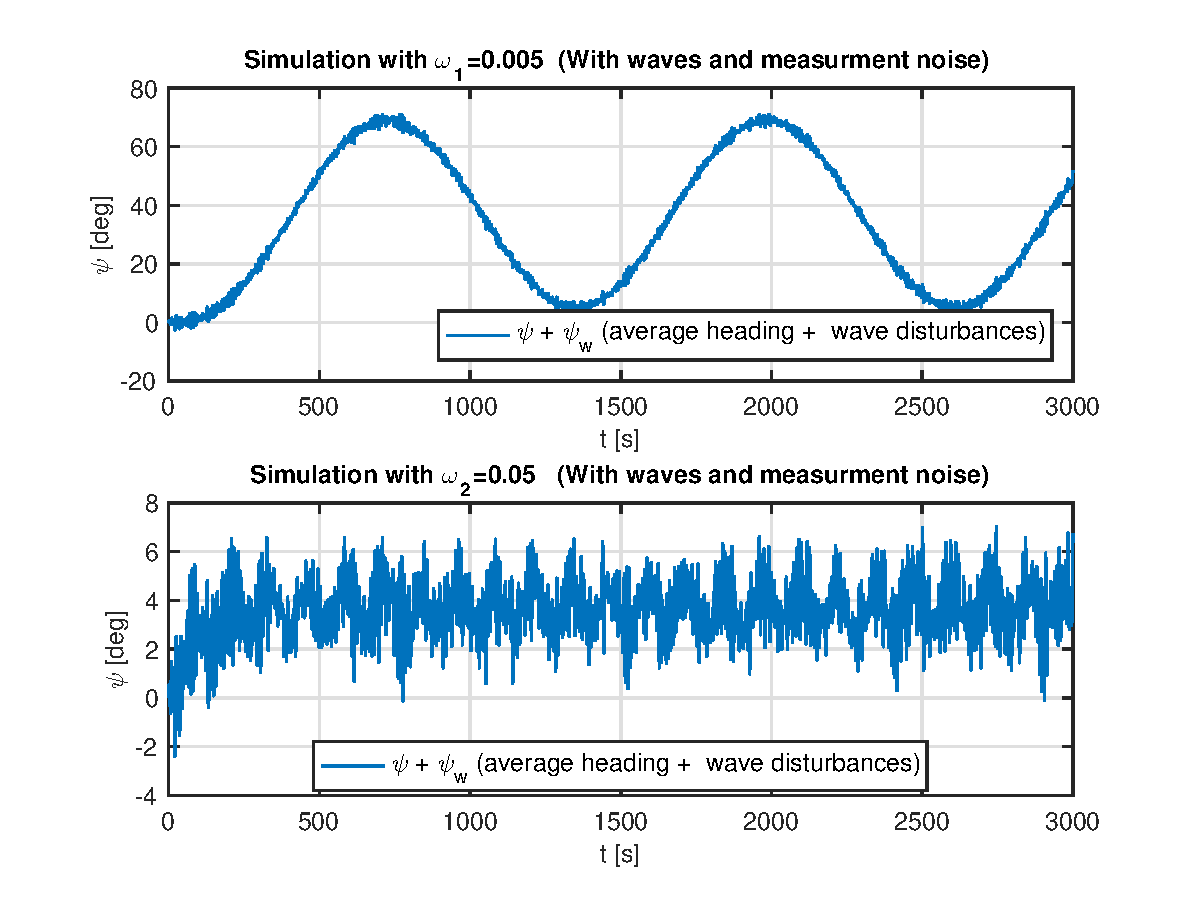
\includegraphics[scale=0.8]{plots/1cA1}}
\end{figure}




From the figure, it is rather difficult to extract any data thus the signal of the noise ratio is low. It is possible though, by using different software tools inside MatLab, but increasing the amplitude of the input signal provided us with the necessary results. An output signal with less noise is obtained by using the following parameters:

\begin{align*}
\omega_1 &= 0.005\\
\omega_2 &= 0.05\\
A &= 45
\end{align*}


\begin{figure}[!htb]
    \caption{Compassion with higher amplitude, A=45}
    \centering
    \centerline{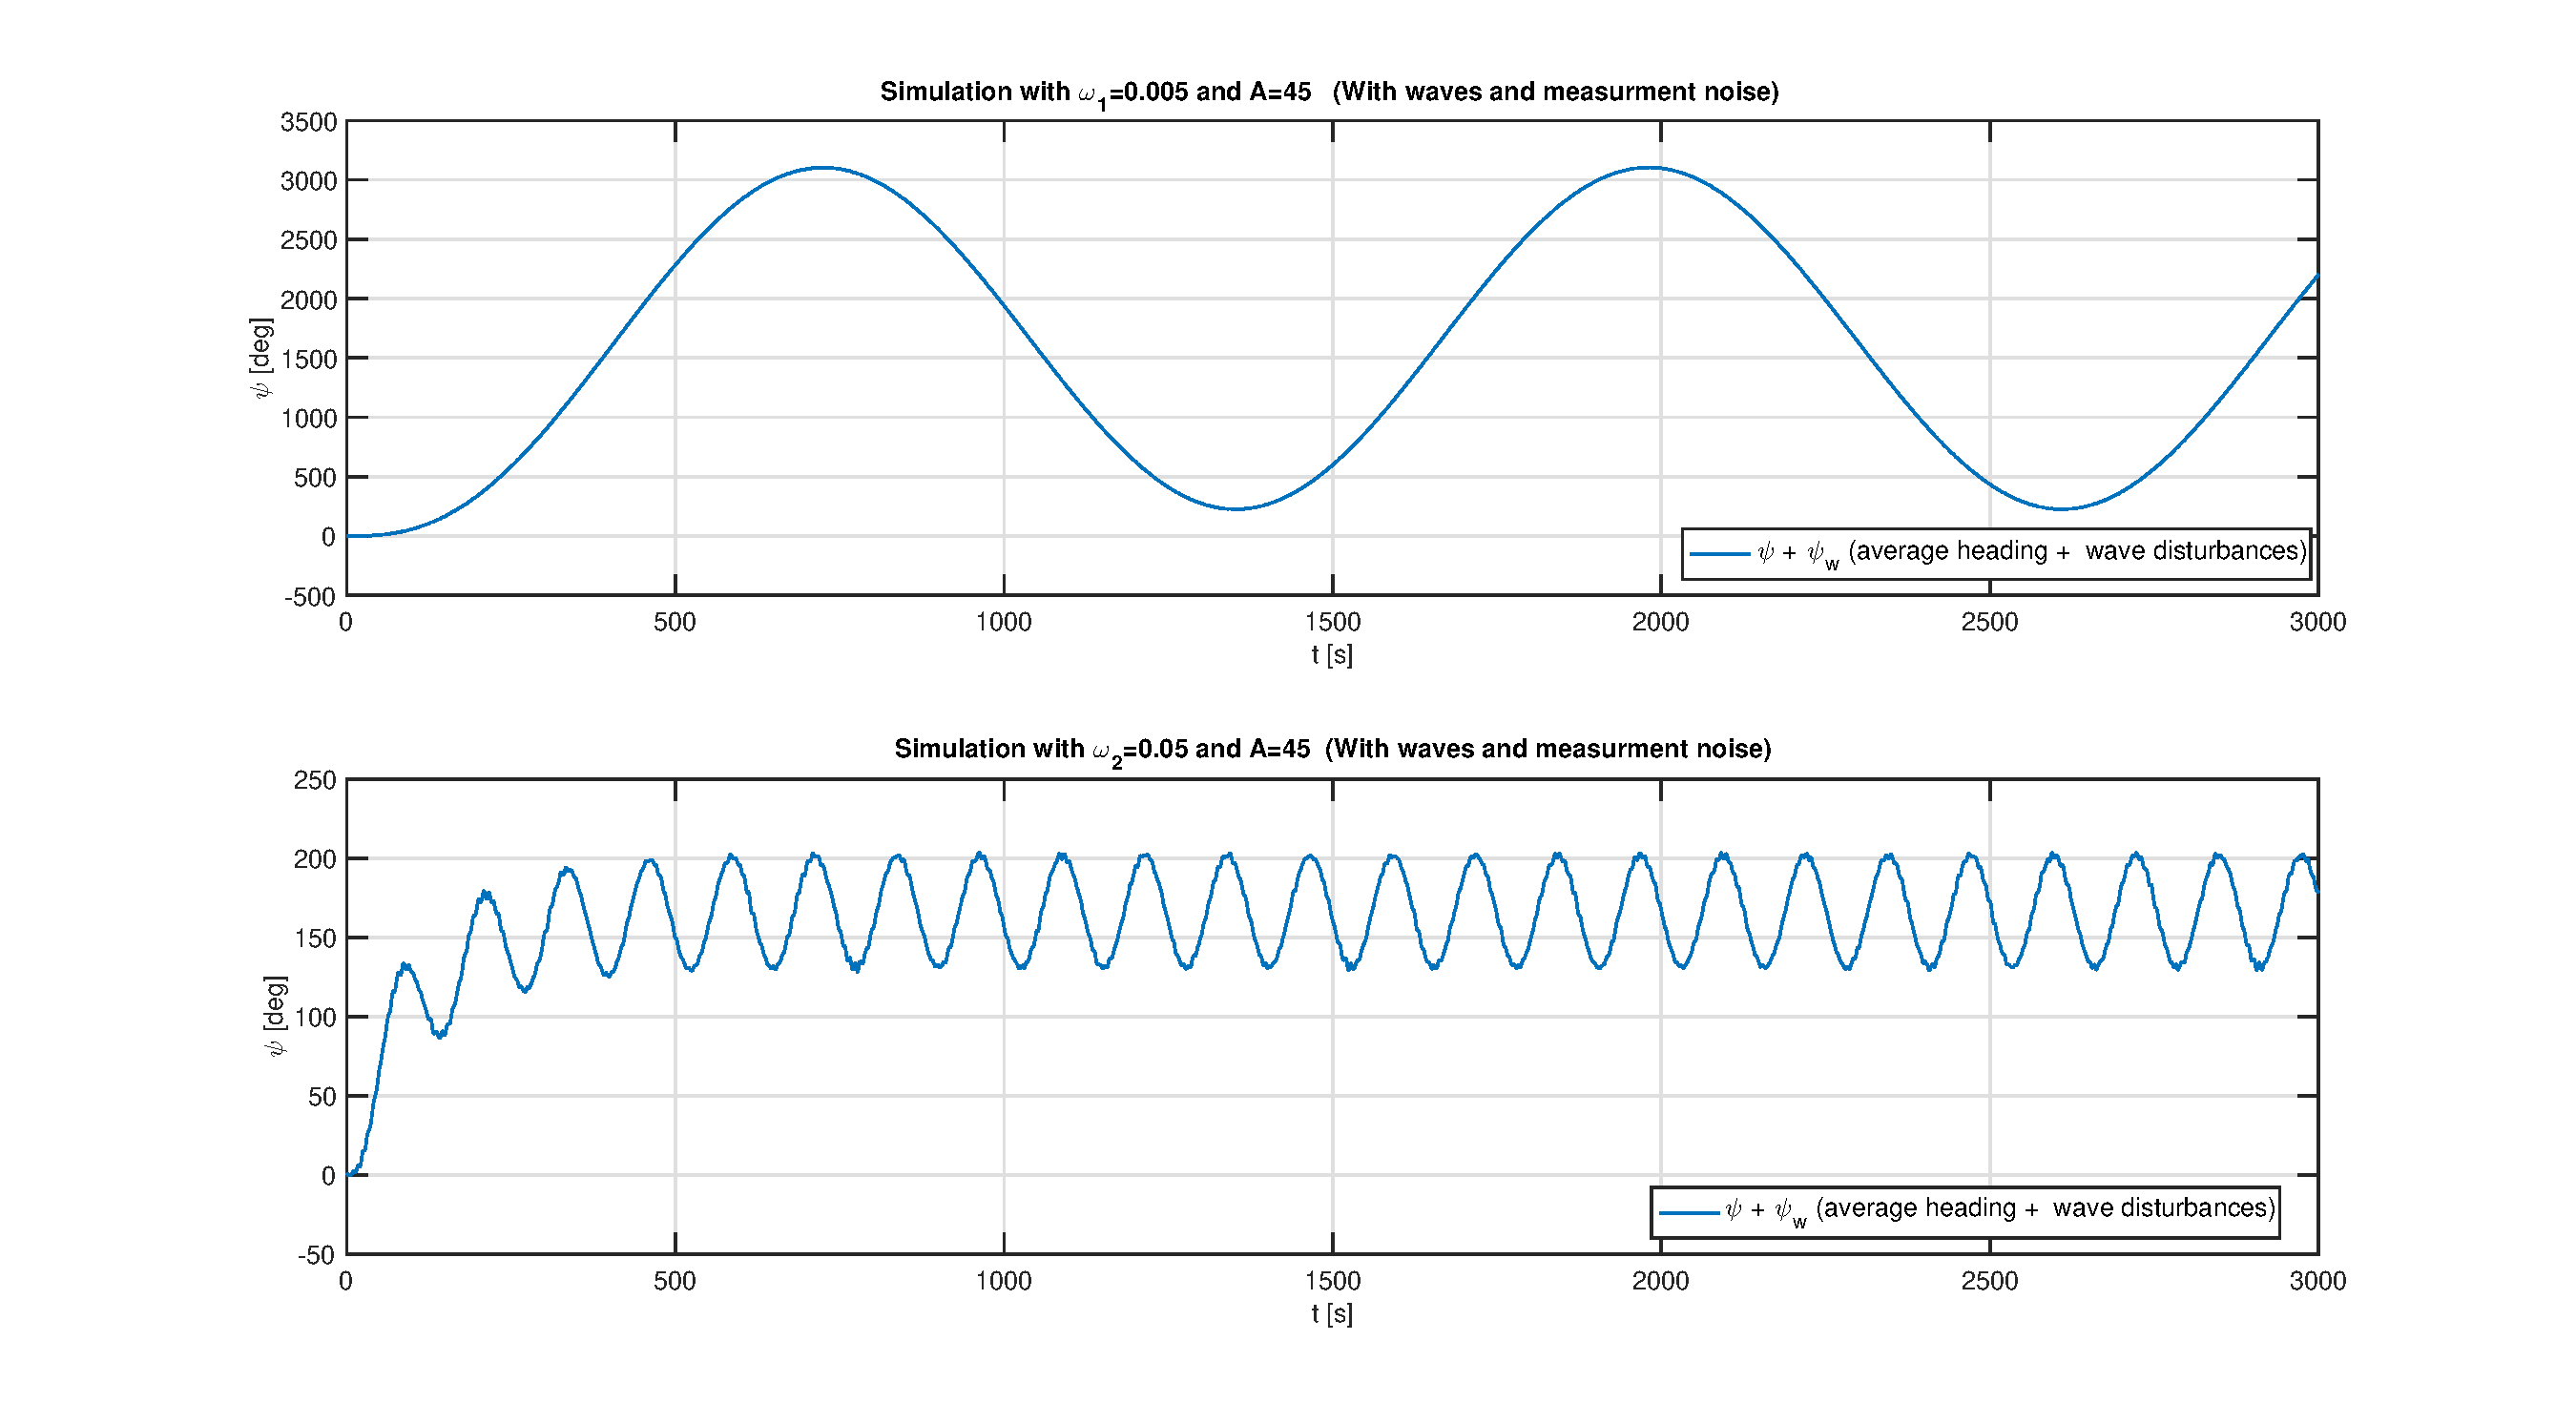
\includegraphics[scale=0.4]{plots/1cA45}}
\end{figure}

These new figures displays a readable format, which is used to calculate the amplitude of the outputs, respectively $A_{01}$ and $A_{02}$.

\begin{align*}
{A_{{0_1}}}  &= \frac{{3105 - 224.5}}{2} = 1440.25\\
{A_{{0_2}}} &= \frac{{202.5 - 130.4}}{2} = 36.05
\end{align*}

Inserting these values into equation (\ref{T}) and equation (\ref{K_calc}) gives:

\begin{align*}
K  &= 0.1734\\
T &= 84.3920
\end{align*}

Comparing these values to what we obtained in section 1.2, we see that the deviation is rather small, less than 2.5\%. The values obtained in section 1.2 are the values that will be used throughout this report.

%%%%%%%%%%%%%%%%%%%%%%%%%%%%%%%%%%%%%%%%%%%%%%%%%%%%%%%%%%%%%%%%%%%%%%%%
% 1.4 Verifying Model Approximation
%%%%%%%%%%%%%%%%%%%%%%%%%%%%%%%%%%%%%%%%%%%%%%%%%%%%%%%%%%%%%%%%%%%%%%%%
\subsection{Verifying Model Approximation}

Figure 4 compares the average heading response $\psi(t)$ of the ship simulation model compared to the estimated model with and without disturbances as a way of simulating weather conditions. The plot shows a good approximation, though the deviation increases with time. Analyzing the plot, it is clear that there is something happening between 300 and 500 seconds, after this the deviation increases and the approximation starts to drift as $t \to \infty $.



%\ref{plot:1d} is displaying the error (${e_\psi }$) of the model compared to the ship. After 450 seconds, error is increasing. $\psi (t)$ is obtained by integrating the yaw rate $r(t)$. Since the comparison displays a good match for at least 450 seconds, we can conclude that the estimated parameters provides a good realistic picture for $r(s)/\delta(s)$.%


\begin{figure}[!htb]
    \caption{Compassion  of model and system}
    \centering
    \centerline{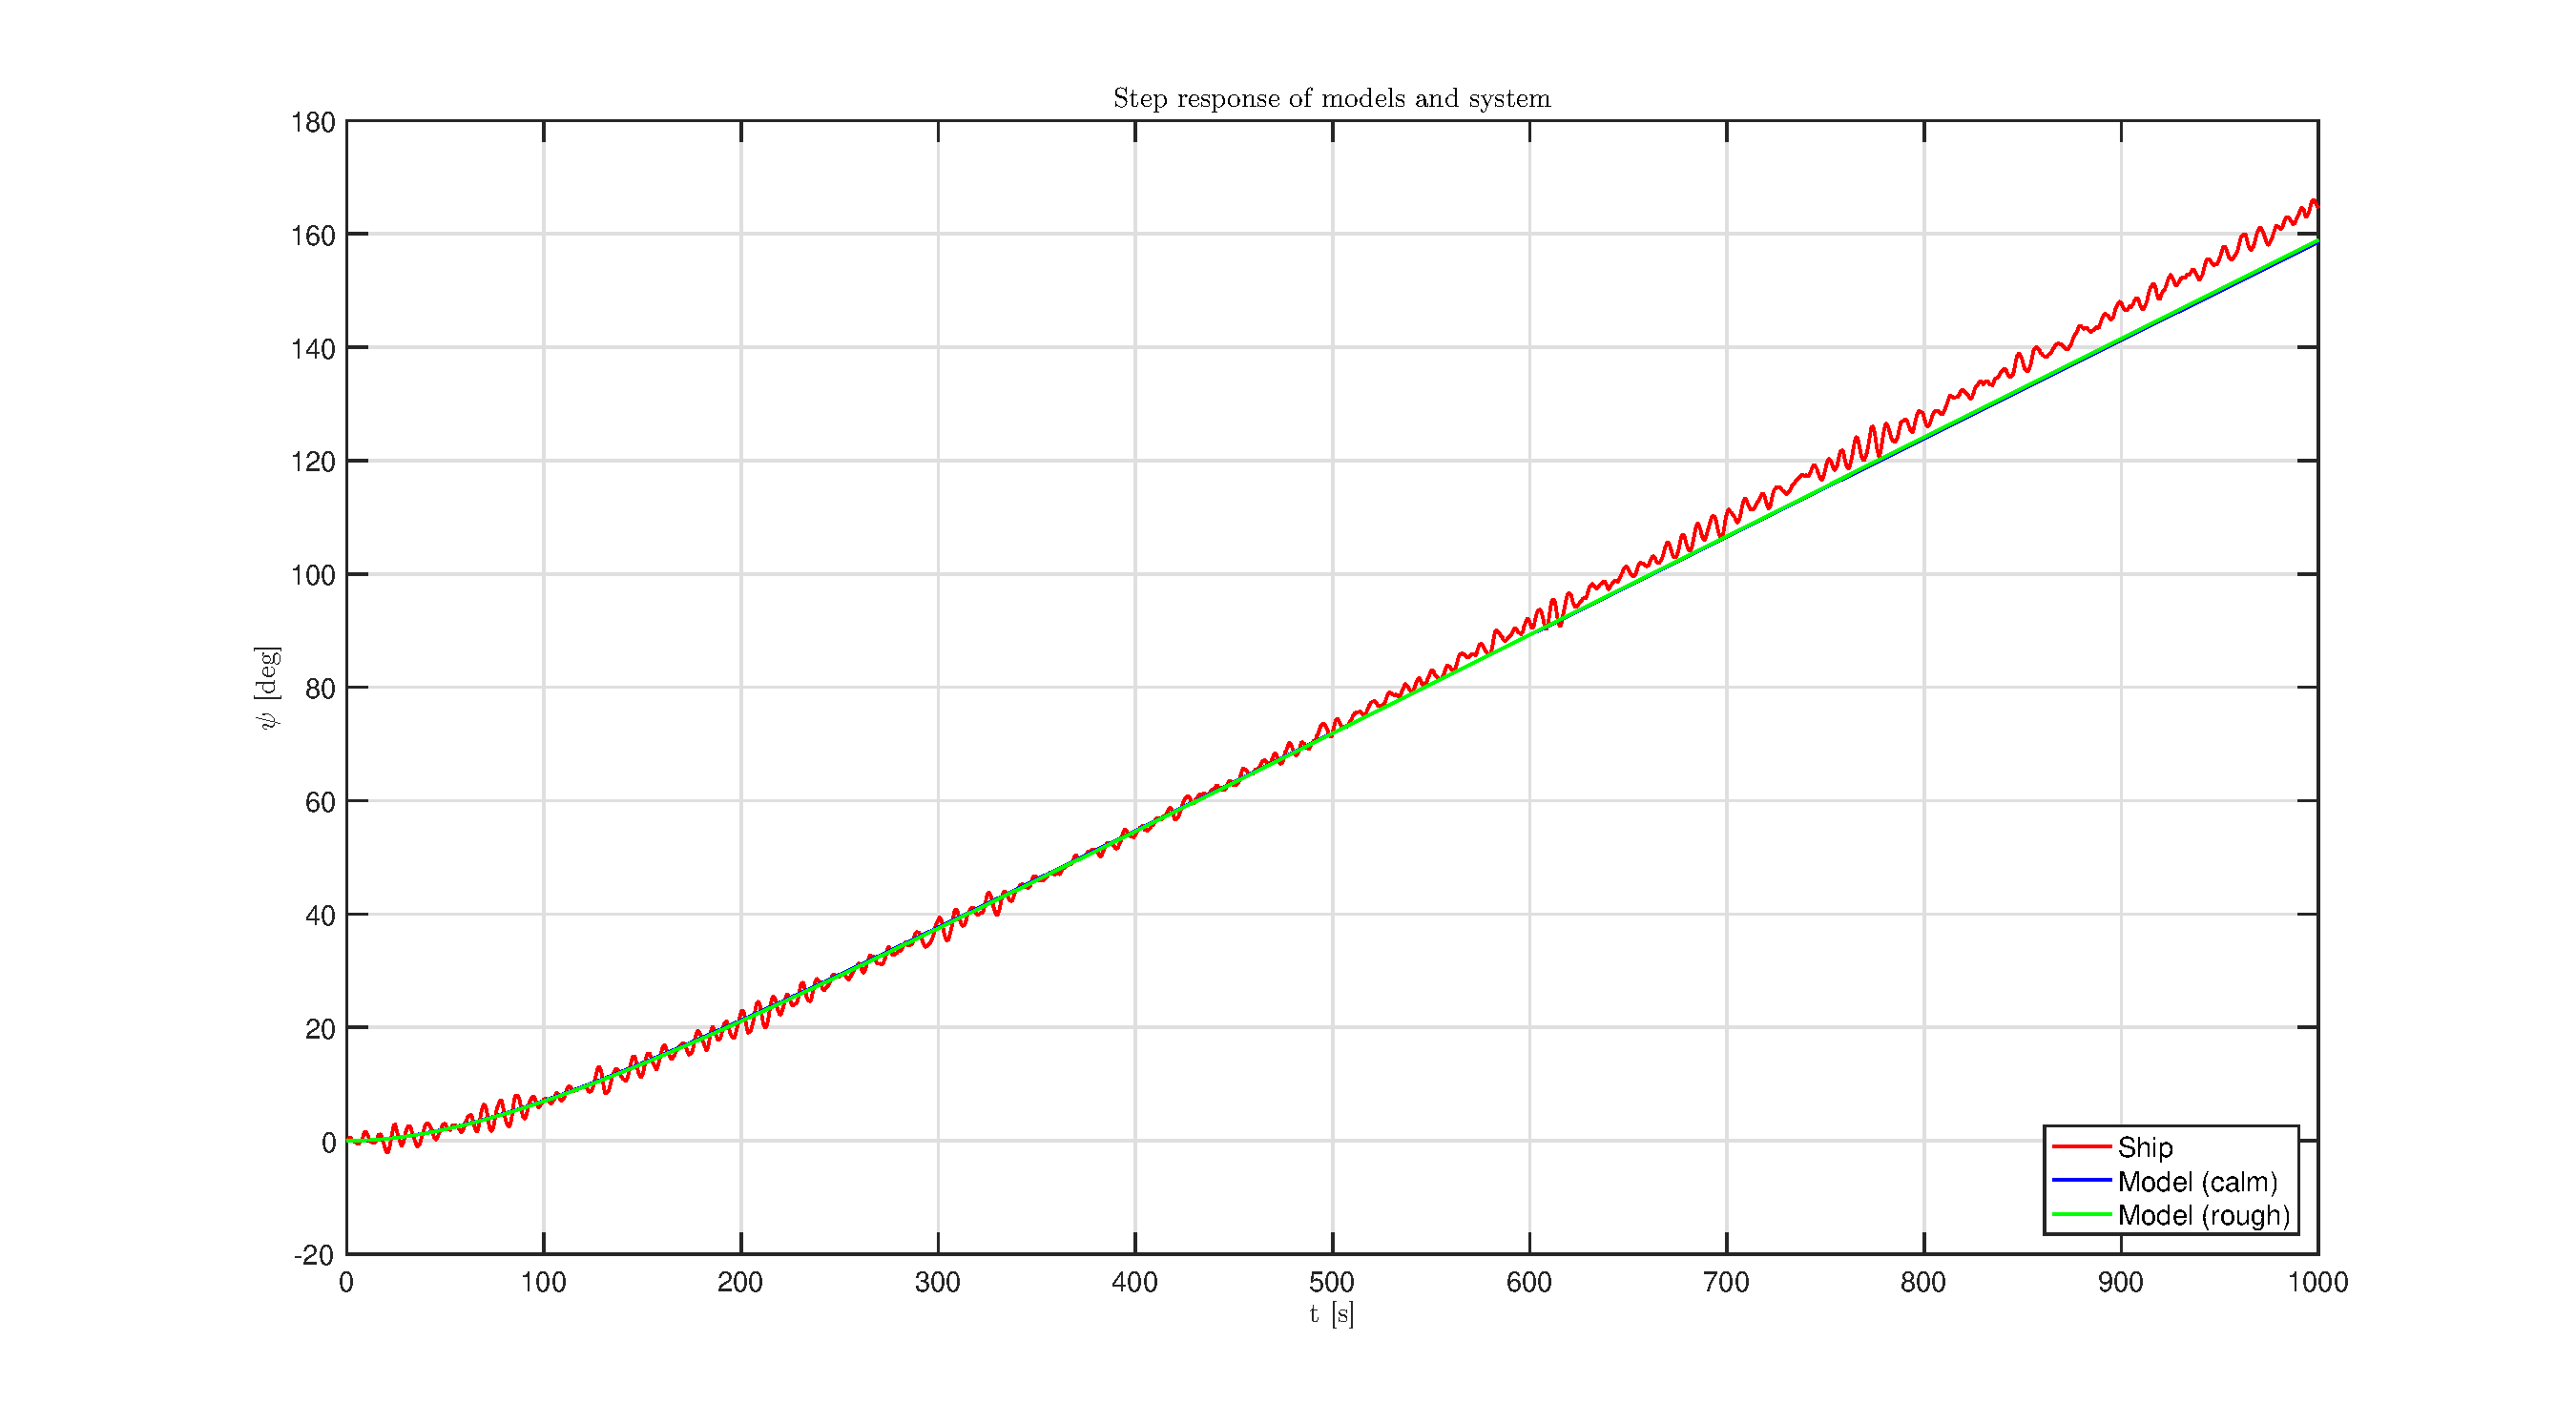
\includegraphics[scale=0.4]{plots/1d}}
    \label{plot:1d}
\end{figure}
